\section{Introduction}
\label{sec:introduction}

The proliferation of cloud storage services is changing the way we think about
wide-area application design. Developers today do not need to build an
application storage solution up-front, but may instead adopt a built-from-parts
design strategy by combining multiple existing storage services. While this
reduces the up-front development cost, this is not sustainable in the long run
since services continuously fail and unilaterally introduce breaking changes
without warning. This paper presents a sustainable approach to synthesizing
stable wide-area storage from unstable storage providers by separating storage
features from providers.

Reusing existing software to create new software is generally good practice.
However, keeping an application working in the face of chronic service
instability is a standing cost, which has proven onerous enough in practice that
many developers end up building their own internal app-specific storage in the
long run. This not only duplicates effort and bugs, but also creates data silos,
whereby the developer is liable for hosting and controlling all I/O on user
data.

\begin{figure}[h!]
\centering
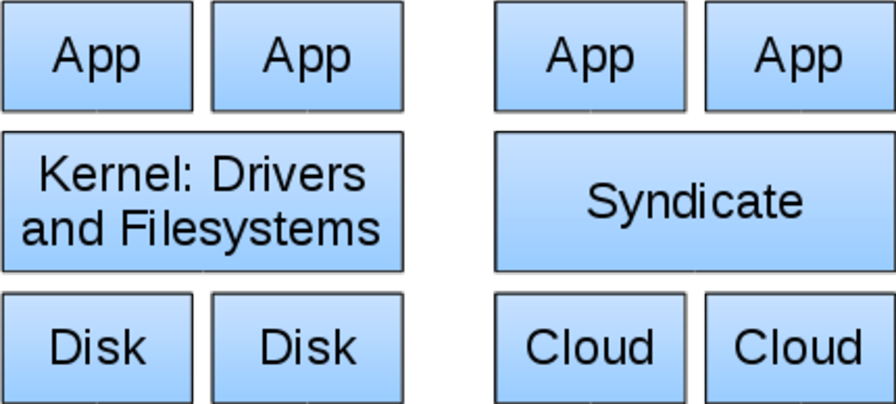
\includegraphics[width=0.5\textwidth]{figures/kernel}
\caption{\it Syndicate fulfills the same relationship between wide-area
applications and storage services as an OS kernel does for userspace and storage
hardware. }
\label{fig:kernel}
\end{figure}

Ideally, we would treat storage services like dumb, interchangeable disks. Then,
we could create a shared ``kernel'' layer between applications and services
(Figure~\ref{fig:kernel}, where we could replace or mask faulty services
on-the-fly and implement desired storage features independently of services.
However, constructing such a layer for wide-area storage services is uniquely
challenging for several reasons:


\textbf{Storage is data-dependent}. Wide-area storage spans multiple
administrative domains, but deciding which domain may store data and how it may
do so both depend on the data itself. For example, financial records must leave
an audit trail, and medical records in the US must conform to HIPPA. Because of
this, the kernel layer needs a separate user-facing control-plane that is
expressive enough to enforce these constraints independent of applications and
services.

\textbf{Data is user-centric}. Users are the sources and sinks for data, and
applications are tools for user-to-user communication. As such, the layer should
give users the ability to control end-to-end how their data is made available
without relying on applications and services.

\textbf{Storage is asynchronous}. Some storage features require an external
actor to implement correctly, such as migrating cold data to long-term storage
and deleting data after a maximum retention period. The layer must support this
notion of asynchronous execution.

\textbf{Users only trust users}. Users need to authenticate data without
trusting the application or the services, but cannot reliably manage credentials
like public keys. The layer must not only respect a users' trust domains, but
also implement a secure and automatic solution for public key discovery and
revocation.

We can overcome these challenges if we reason about how the end-to-end I/O flows
(e.g. reads and writes) pass through services and applications.  We observe that
the shared layer's functionality is composed of multiple \textit{execution contexts}
which each perform a stateful transformation on a flow before passing it along
such as replication or logging (Figure~\ref{fig:execution-contexts}).  By
considering the sequence of transformations applied on each I/O flow as it
travels from one user to another, we can describe a \textit{global I/O
coordination algorithm} that runs in this layer and defines the aggregate
storage behavior to applications.

\begin{figure}[t!]
\centering
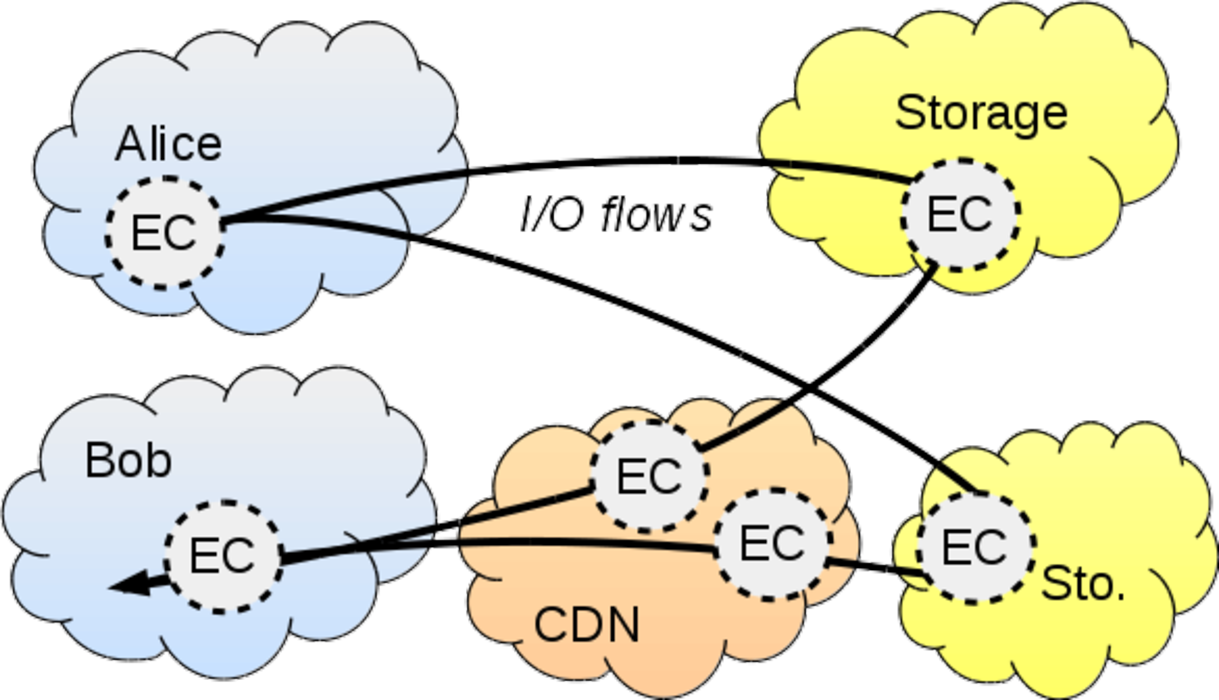
\includegraphics[width=0.5\textwidth]{figures/execution-contexts}
\caption{\it In built-from-parts wide-area applications today, Alice's writes
and Bob's reads can be thought of as data flows that implicitly pass through
multiple execution contexts (ECs) in each service.  The ECs
implement all stateful transformations on user data, thereby defining
precisely the storage features available to the application.}
\label{fig:execution-contexts}
\end{figure}

We argue that all of the functionality in this layer is already present in
applications today, but is very hard to reason about because it is an implicit
cross-cutting concern. However, execution contexts and the global I/O
coordination algorithm precisely characterize the storage features, which make
them worthy of independent study.

The contribution of this paper is to show how to construct this wide-area kernel
layer in terms of I/O flows, execution contexts, and the global I/O coordination
algorithm. Our approach is analogous to how SDN separates networks from
infrastructure by building a ``network kernel'' that composes flow rules to
create an app-defined global network topology. In our approach, we separate
storage features from providers by building a ``storage kernel'' that
composes storage logic running in execution contexts to create an app-defined
global I/O coordination algorithm.

We use the term \textit{software-defined networked storage (SDNS)} to refer to this
design paradigm.  To demonstrate the concept, we created a file-oriented SDNS
system called Syndicate. Syndicate offers a programmable data-plane that gives
users control over how a set of Syndicate-controlled execution contexts handle
I/O flows on their files.  Its key novelty is that it leverages an existing
blockchain to maintain a global, consistent view of its execution contexts
without introducing a single point of trust. This is critical to maintaining a
distributed control plane that spans multiple administrative and trust domains.
By doing so, Syndicate offers a generic way to implement storage features on
top of existing storage systems in a reusable manner, giving applications stable
but custom storage built on existing systems as if they were dumb,
interchangeable disks.
